\documentclass[11pt,a4paper]{article}
\usepackage[utf8]{inputenc}
\usepackage[german]{babel}
\usepackage[T1]{fontenc}
\usepackage{amsmath}
\usepackage{amsfonts}
\usepackage{amssymb}
\usepackage{graphicx}
\usepackage[margin=1.25cm]{geometry} % Puts the same margin on all borders of the document

% Packages

\usepackage{hyperref} % Generate hyperlinks to referenced items
\usepackage{adjustbox} % Used to change parameters in \includegraphics[scale=•]{•}
\usepackage{enumitem} % Provides several options for lists
\usepackage{verbatim} % Package to use \begin{comment}
\usepackage{pdfpages} % Used to import PDF pages
\usepackage{multirow} % Allows us to have a single cell in a table span multiple rows
\usepackage{makecell} % Allows us to format multiple lines in a single cell
\usepackage{minted} % Used to syntax highlight code
\usepackage{xcolor}  % Gives access to coloring text
\usepackage{longtable} % Allows us to create a table over multiple pages
\usepackage{float} % Improved placement of floating items
\usepackage{pdfpages} % Used to import pdf pages
\usepackage{booktabs} % Used for horizontal lines instead of \hline



% Settings

\graphicspath{{./files/}} % Sets path for files to the files folder in the same directory

\hypersetup{
    colorlinks=false, %set true if you want colored links
    linktoc=all,     %set to all if you want both sections and subsections linked
    linkcolor=blue,  %choose some color if you want links to stand out
}


\renewcommand{\arraystretch}{1.75} 

\lstset {
	literate={~} {$\sim$}{1},
    language=Java,
    basicstyle=\footnotesize,
    numbers=left,
    stepnumber=1,
    showstringspaces=false,
    tabsize=1,
    breaklines=true,
    breakatwhitespace=false,
    inputencoding=utf8,
    extendedchars=true   
}

\begin{titlepage}
  \title{FOP Reference Sheet} % document_name-type_of_document
  \author{Jonas Milkovits}
  \date{Last Edited: \today}
\end{titlepage}

\begin{document}

\pagenumbering{gobble}
\maketitle
\pagenumbering{roman} % i, ii, iii on beginning pages, that don't have content
\tableofcontents
\clearpage
\pagenumbering{arabic} % 1,2,3 on content pages

\begin{comment}
	\begin{tabular}{ | p{4cm} p{13.5cm} | }
	\hline
	\makecell[l]{} & \makecell[l]{$\rhd$  } \\ \hline
	
	\makecell[l]{} & \makecell[l]{$\rhd$  } \\ \hline
	
	\makecell[l]{} & \makecell[l]{$\rhd$  } \\ \hline
	
	\makecell[l]{} & \makecell[l]{$\rhd$  } \\ \hline
	
	\makecell[l]{} & \makecell[l]{$\rhd$  } \\ \hline
	
	\makecell[l]{} & \makecell[l]{$\rhd$  } \\ \hline
	
	\makecell[l]{} & \makecell[l]{$\rhd$  } \\ \hline

	\makecell[l]{} & \makecell[l]{$\rhd$  } \\ \hline
	
	\end{tabular}
\end{comment}


\section{Stuff that I skipped cuz of chapter 4}

\begin{tabular}{ | p{4cm} p{13.5cm} | }
	\hline
	\makecell[l]{Exceptions aus \\ Lambda-Ausdrücken} &
	\makecell[l]{$\rhd$ Kapitel 5: 47 - 50  } \\ \hline
	
	\makecell[l]{} & \makecell[l]{$\rhd$  } \\ \hline
	
	\makecell[l]{} & \makecell[l]{$\rhd$  } \\ \hline
	
	\makecell[l]{} & \makecell[l]{$\rhd$  } \\ \hline
	
	\makecell[l]{} & \makecell[l]{$\rhd$  } \\ \hline
	
	\makecell[l]{} & \makecell[l]{$\rhd$  } \\ \hline
	
	\makecell[l]{} & \makecell[l]{$\rhd$  } \\ \hline

	\makecell[l]{} & \makecell[l]{$\rhd$  } \\ \hline
	
	\end{tabular}

\section{Computerspeicher}



	\begin{tabular}{ | p{4cm} p{13.5cm} | }
	\hline
	\makecell[l]{Unsere Vorstellung} & 
	\makecell[l]{$\rhd$ großes Feld aus Maschinenwörtern mit eindeutiger Adresse} \\ \hline
	
	\makecell[l]{Erzeugung eines \\ neuen Objekts} & 
	\makecell[l]{$\rhd$ Reservierung von ungenutztem Speicher in ausreichender Größe} \\ \hline
	
	\makecell[l]{Referenz} & 
	\makecell[l]{$\rhd$ Name der Variable, die die Anfangsadresse des Objekts speichert \\ 
	$\rhd$ Kann auch an komplett anderer Stelle als das Objekt gespeichert sein } \\ \hline
	
	\makecell[l]{Speicherort primitiver \\ Datentypen} & 
	\makecell[l]{$\rhd$ Name verweist tatsächlich auf Speicherstelle, an der Wert abgespeichet wird } \\ \hline
	
	\makecell[l]{Prozessablauf} & 
	\makecell[l]{$\rhd$ Program Counter enthält Adresse der nächsten Anweisung \\
	\hspace{0.4cm} $\diamond$ Zählt nach jeder Anwendung hoch und verweist auf nächsten Speicher \\
	$\rhd$ CPU verarbeitet parallel die momentane Anweisung aus Program Counter} \\ \hline
	
	\makecell[l]{Methodenausführung} & 
	\makecell[l]{$\rhd$ Einrichtung einer Variable \texttt{StackPointer} bei Programmstart \\
	$\rhd$ StackPointer enthält die Adresse des \texttt{Call-Stacks} \\
	$\rhd$ Bei Methodenaufruf wird im Speicher Platz reserviert, genannt \texttt{Frame} \\
	$\rhd$ \texttt{Frame}  wird dann auf dem Call-Stack abgelegt\\
	$\rhd$ Der \texttt{StackPointer}  wird dann mit der Adresse des neuen\texttt{Frames}  überschrieben \\
	$\rhd$ Methodenaufruf vorbei: Frame wird wieder vom \texttt{Call-Stack} genommen \\
	$\rhd$ \texttt{StackPointer} wird auf Adresse des vorherigen \texttt{Frames}  gesetzt} \\ \hline
	
	\makecell[l]{Methodentabelle} & \makecell[l]{$\rhd$ Enthält bei Objekt die Anfangsadressen der 
	verfügbaren Methoden } \\ \hline
	
	\end{tabular}
	
	\begin{center}
	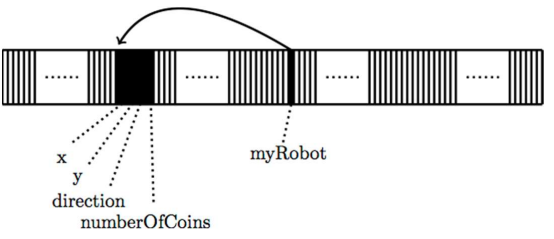
\includegraphics[scale=0.8]{computerspeicher}
	\end{center}

\section{Datenstrukturen}

\begin{tabular}{ | p{4cm} p{13.5cm} | }
	\hline
	\makecell[l]{Array} & 
	\makecell[l]{$\rhd$ Verwendet zum Speichern von mehreren Variablen des selben Typs \\
	$\rhd$ Erzeugung: \texttt{int[] test = new int[n];} \\
	$\rhd$ \texttt{n} gibt in diesem Fall die feste Anzahl der speicherbaren Variablen an \\
	$\rhd$ Natürlich auch Arrays von Objekten möglich \\
	$\rhd$ Zugriff auf Variablen: \texttt{test[0]} für ersten Wert (Index) \\
	$\rhd$ Zugriff auf Länge: \texttt{test.length} } \\ \hline
	\end{tabular}



\section{Datentypen}

	\begin{tabular}{ | p{4cm} p{13.5cm} | }
	\hline
	\makecell[l]{Konstanten} & \makecell[l]{$\rhd$ Variable/Referenz wird dadurch unveränderbar \\
	$\rhd$ z.B.: \texttt{final myClass ABC = new myClass();} \\
	\hspace{0.4cm} $\diamond$ Referenz zwar nicht veränderbar, Objekt aber schon \\ 
	$\rhd$ \texttt{Integer.MAX\_VALUE / Integer.MIN\_VALUE} \\
	$\rhd$ Unendlich: \texttt{Double.POSITIVE\_INFINITY / Double.NEGATIVE\_INFINITY} \\
	$\rhd$ Müssen initalisiert werden } \\ \hline
	
	\makecell[l]{Primitive Dateitypen} & 
	\makecell[l]{$\rhd$ Ganze Zahlen: byte $\rightarrow$ short $\rightarrow$ int $\rightarrow$ long \\
	$\rhd$ Gebrochene Zahlen: float $\rightarrow$ double \\
	$\rhd$ Logik: boolean \\
	$\rhd$ Zeichen: char \\
	$\rhd$ Mehrere Definitonen: \texttt{int m = 1, n, k = 2;} \\ 
	$\rhd$ Ohne Initialisierung: undefinierter Wert} \\ \hline
	
	\makecell[l]{Literale} & \makecell[l]{$\rhd$ wörtlich hingeschriebene Werte eines Datentyps  \\
	$\rhd$ Zahlen standardmäßig int, falls \texttt{long} gewünscht: \texttt{123L oder 123l} \\ 
	$\rhd$ Bei gebrochenen double, falls \texttt{float} gewünscht: \texttt{12.3F oder 12.3f} \\
	$\rhd$ null: Nutzung für Referenzen $\rightarrow$ verweist auf nichts} \\ \hline
	
	\makecell[l]{Boolean} & \makecell[l]{$\rhd$ nur \texttt{true} und \texttt{false} \\
	$\rhd$ Negation \texttt{!a} \\
	$\rhd$ Logisches Und: \texttt{a \&\& b} \\
	$\rhd$ Logisches Oder: \texttt{a || b} (inklusiv) \\
	$\rhd$ Gleichheit: \texttt{a == b} } \\ \hline
	
	\makecell[l]{Zeichentyp char} & \makecell[l]{$\rhd$ z.B.: \texttt{char c = ´a´;} \\
	$\rhd$ Interne Kodierung als Unicode \\
	$\rhd$ \textbackslash t Horizontaler Tab \\
	$\rhd$ \textbackslash b Backspace \\
	$\rhd$ \textbackslash n Neue Zeile \\
	$\rhd$ Auch Darstellung im Hexacode (\textbackslash u039A)} \\ \hline
	
	\makecell[l]{Enumeration} & \makecell[l]{$\rhd$ Zusammenfassung mehrerer Konstanten (feste Anzahl)\\
	$\rhd$ Erzeugung meist in eigener .java Datei \\
	$\rhd$ \texttt{enum MyDirection \{DOWN, RIGHT\} } \\
	$\rhd$ Keine Objekterzeugung von Enumeration möglich \\
	$\rhd$ Abspeichern in Variable des Enum-Types ist jedoch möglich \\
	$\rhd$ \texttt{MyDirection dir = MyDirection.DOWN;} \\
	$\rhd$ Klassenmethoden: \\
	\hspace{0.4cm} $\diamond$ \texttt{values() // Returns array with all enum components} \\
	\hspace{0.4cm} $\diamond$ \texttt{name() // Returns the name of the calling object as string} \\
	 } \\ \hline
	
	\makecell[l]{Referenztypen} & \makecell[l]{$\rhd$ Alle Typen, die keine primitiven Datentypen sind \\
	$\rhd$ Unterscheidung zwischen Referez und eigentlichem Objekt \\
	$\rhd$ Gleichheitsoperator \texttt{==} vergleicht nur die Referenz (Objektidentität) \\
	\hspace{0.4cm} $\diamond$ Verweis auf dasselbe Objekt \\
	$\rhd$ Wertgleichheit bezieht sich auf das Objekt an sich \\
	\hspace{0.4cm} $\diamond$ Deep Copy $\Rightarrow$ An allen parallelen Stellen Wertgleichheit \\
	\hspace{0.4cm} $\diamond$ Shallow Copy $\Rightarrow$ Nur Kopie der Adressen \\
	$\rhd$ Ohne Initialisierung: Null} \\ \hline
	\end{tabular}


\section{Exceptions (java.lang.Exception;)}

\begin{tabular}{ | p{4cm} p{13.5cm} | }
	\hline
	\makecell[l]{Exception-Klassen} & \makecell[l]{$\rhd$ Alle Klassen, die direkt oder indirekt von java.lang.Exception abgeleitet sind \\
	$\rhd$  } \\ \hline

	\makecell[l]{Exception werfen} & \makecell[l]{$\rhd$ \texttt{throws Exception \{...\}} nach Parameterliste im Methodenkopf \\
	$\rhd$ Dies signalisiert, dass die Methode mindestens einen Fehler wirft \\
	$\rhd$ Die geworfene Exception muss vom \texttt{throws}-Typ oder Subtyp sein \\
	$\rhd$ Auch mehrere Exceptions möglich, mit einem Komma getrennt \\
	$\rhd$ Werfen der Exception: \\
	\hspace{0.4cm} $\diamond$ z.B.: \texttt{throw new Exception ("No lower case letter!");} \\
	\hspace{0.4cm} $\diamond$ Hier wird als Parameter für die Objekterstellung ein String übergeben \\
	$\rhd$ \texttt{throws}: \\
	\hspace{0.4cm} $\diamond$ Führt zur Beendung der Methode \\
	\hspace{0.4cm} $\diamond$ Liefert das geworfene Exception-Objekt zurück } \\ \hline

	\makecell[l]{Exception fangen} & \makecell[l]{$\rhd$ Bei Methoden, die Exceptions werfen, wird ein \texttt{try-catch}-Block benötigt \\
	$\rhd$ Aufbau: \\
	\hspace{0.4cm} $\diamond$ Methoden, die Exceptions werfen in \texttt{try \{...\}} aufrufen \\
	\hspace{0.4cm} $\diamond$ Falls Exception auftritt wird \texttt{catch (Exception exc) \{...\}} aufgerufen \\
	\hspace{0.4cm} $\diamond$ \texttt{catch} muss direkt im Anschluss nach \texttt{try} stehen \\
	\hspace{0.4cm} $\diamond$ Falls kein Fehler auftritt, wird \texttt{catch} übersprungen \\
	\hspace{0.4cm} $\diamond$ Das Programm wird dann normal weiter ausgeführt \\
	$\rhd$ Es sind auch mehrere \texttt{catch}-Blöcke mit versch. Parametern möglich \\
	$\rhd$ Methoden: \\
	\hspace{0.4cm} $\diamond$ \texttt{getMessage(); // Returns the error message as a string} \\
	\hspace{0.4cm} $\diamond$ \texttt{printStackTrace(); // Ausgabe des Call-Stacks} \\
	$\rhd$ Alle möglichen Exceptions müssen durch den \texttt{catch}-Block abgedeckt sein \\
	$\rhd$ Falls Exception zu mehreren \texttt{catch}-Blöcken 'passt', wird der Erste ausgeführt \\
	\hspace{0.4cm} $\diamond$ Deswegen Reihung der \texttt{catch}-Blöcke von Subtyp nach Supertyp \\
	$\rhd$ Auch mehrere Exceptions in einem \texttt{catch}-Block möglich mit \texttt{||}} \\ \hline

	\makecell[l]{Weiterreichen} & \makecell[l]{$\rhd$ Weiterreichen der Fehlermeldung durch \texttt{throws} im Methodenkopf möglich \\
	$\rhd$ Kein \texttt{try-catch}-Block notwendig \\
	$\rhd$ Main-Methode kann z.B. keine Exceptions weiterreichen} \\ \hline

	\makecell[l]{ \texttt{try-with-ressources} } & \makecell[l]{$\rhd$ Für Ressourcen, die unbedingt wieder geschlossen werden müssen \\
	$\rhd$ Öffnung der Ressource in runden Klammern: \texttt{try (Printer p =... ) \{...\}} \\
	$\rhd$ Mehrere Ressourcen möglich, getrennt durch Semikolon } \\ \hline

	\makecell[l]{Runtime Exceptions} & \makecell[l]{$\rhd$ Ausnahme zu \texttt{try}-Blöcken \\
	$\rhd$ Exceptions von java.lang.RuntimeException und Subtypen \\
	$\rhd$ z.B.: IndexOutOfBoundsException, NullPointerException \\ 
	$\rhd$ Grund: Vermeidung von dauerenden \texttt{try}-Blöcken} \\ \hline
	
	\makecell[l]{Throwable und Error} & \makecell[l]{$\rhd$ Exception und Error sind beide von Throwable abgeleitet \\
	$\rhd$ Alle drei befinden sich im Paket java.lang \\
	$\rhd$ Error: \\
	\hspace{0.4cm} $\diamond$ Werden geworfen, falls Fehlerbehandlung keinen Sinn macht \\
	\hspace{0.4cm} $\diamond$ Programmabbruch als Ausweg \\
	$\rhd$ AssertionError: \\
	\hspace{0.4cm} $\diamond$ \texttt{throw new AssertionError("Bad!");} \\
	\hspace{0.4cm} $\diamond$ Kurzform: \texttt{assert x == 2: "Bad!";} \\
	\hspace{0.4cm} $\diamond$ \textbf{Wichtig:} Bedingung muss negiert werden!
	\hspace{0.4cm} $\diamond$ Assertanweisungen sinnvoll, da kurz und übersichtlich \\
	\hspace{0.4cm} $\diamond$ Können zusätzlich vom Compiler an- und abgeschaltet werden \\
	\hspace{0.4cm} $\diamond$ z.B.: Verwendung für Tests für Methoden und späteres Abschalten \\
	$\rhd$ Solche Tests werden White-Box-Tests genannt } \\ \hline

	\end{tabular}

\section{Fehler}
	\begin{tabular}{ | p{4cm} p{13.5cm} | }
	\hline
	\makecell[l]{Kompilierzeitfehler \\ (compile-time errors)} & 
	\makecell[l]{$\rhd$ Falsche Klammersetzung, falsche Schlüsselwörter,..\\
	$\rhd$ Programm wird nicht übersetzt $\Rightarrow$ Fehlermeldung vom Compiler } \\ \hline
	
	\makecell[l]{Laufzeitfehler \\ (run-time errors)} & 
	\makecell[l]{$\rhd$ Tritt während der Ausführung auf \\
	$\rhd$ Führt zum Abbruch des Programms $\Rightarrow$ Ausgabe der Fehlermeldung \\
	$\rhd$ Kann nicht vom Compiler entdeckt werden \\
	$\rhd$ IndexOutOfBounds, NullPointerException,.. } \\ \hline
	\end{tabular}

\section{Graphics (java.awt.Graphics;)}
	\begin{tabular}{ | p{4cm} p{13.5cm} | }
	\hline
	\makecell[l]{Applet} & \makecell[l]{$\rhd$ leichtgewichtige Variante an Graphikprogrammen \\
	$\rhd$ \texttt{import java.awt.Applet;} \\
	$\rhd$ 1. Erstellen eigener Applet-Klasse (\texttt{extends Applet}) \\
	$\rhd$ 2. Überschreiben der Methode \texttt{paint} \\
	\hspace{0.8cm} \texttt{public void paint (Graphics graphics) \{...\}} \\
	\hspace{0.8cm} Klasse \texttt{Graphics} verknüpft Programm mit Zeichenfläche \\
	$\rhd$ 2.1 \texttt{GeomShape2D}-Array \\
	\hspace{0.8cm} \texttt{GeomShape2D pic = new GeomShape2D[3];} \\
	\hspace{0.8cm} Füllen des erstellten Arrays mit Formen (z.B.: \texttt{ new Circle(0,0,0);})\\
	$\rhd$ 2.2 Erstellen jeder Form mithilfe Randfarbe, Füllfarbe und Zeichnen \\
	\hspace{0.8cm} \texttt{pic[0].setBoundaryColor(Color.RED); // Randfarbe} \\
	\hspace{0.8cm} \texttt{pic[0].setFillColor(Color.RED);	  // Füllfarbe} \\
	\hspace{0.8cm} \texttt{pic[0].paint(graphics); // Eigentliches Zeichnen}} \\ \hline
	
	\makecell[l]{GeomShape2D} & \makecell[l]{$\rhd$ Abstrake Klasse (Methode \texttt{paint} ist abstrakt) \\
	$\rhd$ Attribute: \\
	\hspace{0.4cm} \texttt{int positionX; int positionY; int rotationAngle;} \\
	\hspace{0.4cm} \texttt{int transparencyValue; Color boundaryColor; Color fillColor;} \\
	$\rhd$ Subklassen: \texttt{Rectangle, Circle, StraightLine} } \\ \hline
	\end{tabular}


\section{Interfaces}
	\begin{tabular}{ | p{4cm} p{13.5cm} | }
	\hline
	\makecell[l]{Erzeugung} & \makecell[l]{$\rhd$ Meist in eigener Datei \\
	$\rhd$ \texttt{public interface MyInterface \{...\}} \\
	$\rhd$ Alle Methodes und das Interface \textbf{müssen} \texttt{public} sein \\ } \\ \hline
	
	\makecell[l]{Methoden} & 
	\makecell[l]{$\rhd$ Werden hier nicht implementiert, sondern nur definiert \\
	$\rhd$ \texttt{public} kann weggelassen werden, da ohnehin notwending \\
	$\rhd$ Implementierte Methoden müssen dann auch \texttt{public} sein \\
	$\rhd$ Falls eine der Methoden nicht implementiert wird $\Rightarrow$ Klasse abstrakt} \\ \hline
	
	\makecell[l]{Verwendung} & \makecell[l]{$\rhd$ \texttt{implements MyInterface} nach Klassenname  \\
	$\rhd$ Beliebig viele Interfaces möglich (seperiert durch ,) \\
	$\rhd$ Ein Interface kann mehrere andere Interfaces erweitern (\texttt{extends}} \\ \hline
	\end{tabular}

\section{JUnit-Tests}


\begin{tabular}{ | p{4cm} p{13.5cm} | }
	\hline

	\makecell[l]{Allgemein} & \makecell[l]{$\rhd$ Tests als Ganzes - Black-Box-Tests \\
	$\rhd$ JUnit-Tests werden in eine seperate Quelldatei geschrieben \\
	$\rhd$ Die zu testende Einheit/Klasse wird dann importiert } \\ \hline

	\makecell[l]{Imports} & \makecell[l]{
	$\rhd$ \texttt{import static org.junit.Assert.assertEquals;} \\
	$\rhd$ \texttt{import static org.junit.Assert.asserTrue;} \\
	$\rhd$ \texttt{import org.junit.jupiter.api.Test;} \\
	$\rhd$ \texttt{import org.junit.jupiter.api.BeforeEach;} \\
	$\rhd$ \texttt{import static org.junit.jupiter.api.Assertions.assertThrows;}} \\ \hline

	\makecell[l]{Methoden:} & 
	\makecell[l]{$\rhd$ \texttt{assertEquals(...,...); // \texttt{true}, falls beide Parameter identisch} \\
	\hspace{0.4cm} $\diamond$ Existiert auch mit 3 Parametern, 3. Wert entspricht maximalen Unterschied \\ 
	$\rhd$ \texttt{assertTrue(...); // \texttt{true}, falls der Parameter \texttt{true} ist} \\
	$\rhd$ \texttt{assertThrows(...,...); // Wirft Exception abhängig von Executable} \\
	\hspace{0.4cm} $\diamond$ Erster Parameter zu werfende Exception.class \\
	\hspace{0.4cm} $\diamond$ Zweiter Paramter Functional Interface aus dem Package java.lang.reflect } \\ \hline
	
	\makecell[l]{Test} & 
	\makecell[l]{$\rhd$ \texttt{@Test} vor der Methode \\
	$\rhd$ \texttt{void} als Rückgabewert \\
	$\rhd$ Nutzung einer \texttt{assert}-Methode (siehe Methoden)} \\ \hline

	\makecell[l]{BeforeEach} & \makecell[l]{$\rhd$ \texttt{@BeforeEach} vor der Methode \\
	$\rhd$ Wird vor jeder einzelnen Testmethode einmal ausgeführt  } \\ \hline
	
	
	
	\end{tabular}

\section{Klassen}

	\begin{tabular}{ | p{4cm} p{13.5cm} | }
	\hline
	\makecell[l]{Erzeugung} & \makecell[l]{$\rhd$ meist in seperater .java Datei  \\
	$\rhd$ \texttt{public class MyClass \{\}} \\
	$\rhd$ \texttt{new MyClass();}: \\
	\hspace{0.4cm} $\diamond$ Reserviert ausreichend Speicherplatz für das Objekt \\ 
	$\rhd$ \texttt{MyClass x = new MyClass();}: \\
	\hspace{0.4cm} $\diamond$ Speichern der Adresse des neuen Objekts in der Referenz x } \\ \hline
	
	\makecell[l]{Attribute} & \makecell[l]{$\rhd$ Eigenschaften der Objekte/Klassen \\
	$\rhd$ z.B.: \texttt{private int x;} (Objektattribut) \\
	$\rhd$ z.B.: \texttt{private static int x;} (Klassenattribut)  } \\ \hline
	
	\makecell[l]{Konstruktor} & 
	\makecell[l]{$\rhd$ Wird zur Erzeugung von neuen Objekten einer Klasse verwendet \\
	$\rhd$ Methode mit selben Namen wie Klasse und ohne Rückgabetyp \\
	$\rhd$ z.B.: \texttt{public MyClass (int x, int y) \{this.x = x; this.y = y;\}} \\
	$\rhd$ Erzeugung eines neuen Objekts: \texttt{MyClass test = new MyClass(2,4);} \\
	$\rhd$ Falls kein Konstruktur angegeben wird $\rightarrow$ Default Constructor \\
	\hspace{0.4cm} $\diamond$ Basisklasse muss auch Konstruktor mit leerer Parameterliste haben \\
	$\rhd$ Konstruktoren werden \texttt{nicht} vererbt \\
	$\rhd$ \texttt{Static Initializer} \\
	\hspace{0.4cm} $\diamond$ Methodenkopf besteht nur aus \texttt{static \{...\}} \\
	\hspace{0.4cm} $\diamond$ Wird genutzt um auf jeden Fall Klassenkonstanten zu initialisieren \\
	$\rhd$ Aufruf anderen Konstruktors in Konstruktor mit \texttt{this(Parameter);}} \\ \hline

	\makecell[l]{Abstraktion} & \makecell[l]{$\rhd$ \texttt{abstract public class MyClass \{...\}} \\
	$\rhd$ Notwendig, sobald Klasse eine abstrakte Methode beinhaltet \\
	$\rhd$ Keine Objekterzeugung möglich \\
	$\rhd$ Meist als Klasse mit Rahmenbedingungen für Subklassen verwendet }  \\ \hline
	
	\makecell[l]{Klasse aller Klassen} & \makecell[l]{$\rhd$ \texttt{java.lang.Object} \\
	$\rhd$ Jede Klasse ist direkt oder indirekt von \texttt{Object} abgeleitet \\
	$\rhd$ Methoden: \\
	\hspace{0.4cm} $\diamond$ \texttt{boolean equals (Object obj) \{...\} // Test auf Wertgleichheit} \\
	\hspace{0.4cm} $\diamond$ \texttt{String toString() \{...\} // Zustand des Objekts als String } \\
	\hspace{0.4cm} $\diamond$ Werden oft an jeweilige Klasse angepasst } \\ \hline
	
	\makecell[l]{Verborgene Informationen} & 
	\makecell[l]{$\rhd$ Jedes Objekt einer Klasse erhält einen Verweis auf ein anonymes Objekt \\
	$\rhd$ Dieses anonyme Objket wird für jede Klasse nur einmal eingerichtet \\
	$\rhd$ Enthät Informatiuonen zur Klasse, Attribute und Methoden der Klasse \\
	$\rhd$ Methodentabelle: \\
	\hspace{0.4cm} $\diamond$ Gibt an, welche Implementationen aller Methoden verwendet wird \\
	\hspace{0.4cm} $\diamond$ Ermöglicht, die Feststellung der Klasse zur Laufzeit \\
	\hspace{0.4cm} $\diamond$ Methode in Supertyp und Substyp haben den selben Index (Position) } \\ \hline
	
	\end{tabular}

\section{Konversionen}

	\begin{tabular}{ | p{4cm} p{13.5cm} | }
	\hline
	\makecell[l]{Implizit} & 
	\makecell[l]{$\rhd$ Immer möglich, wenn kein Informationsverlust entstehen kann \\
	$\rhd$ z.B.: kleinerer Datentyp in größeren } \\ \hline
	
	\makecell[l]{Explizit} & \makecell[l]{$\rhd$ Meist Informationsverlust \\
	$\rhd$ Durchführung durch Angabe des Datentyps in Klammern davor \\
	$\rhd$ z.B.: \texttt{int i = (int)testDouble;} } \\ \hline
	\end{tabular}


\section{Methoden}
	\begin{tabular}{ | p{4cm} p{13.5cm} | }
	\hline
	\makecell[l]{Methodenaufbau} & 
	\makecell[l]{$\rhd$  Modifier Rückgabewert Identifier (Parameterliste) \{Anweisung\} \\
	$\rhd$ Alles vor den Anweisung: Methodenkopf (Head) \\
	$\rhd$ Alles in den geschweiften Klammern: Methodenrumpf (Body) \\
	$\rhd$ z.B.: \texttt{public void setX (int x) \{this.x = x;\}} (Objektmethode) \\
	$\rhd$ z.B.: \texttt{public static void setY (int y) \{this.y = y;\}} (Klassenmethode) \\
	$\rhd$ \texttt{this.x} steht hier für das Objektattribut und nicht den Parameter} \\ \hline
	
	\makecell[l]{Ausführung} & \makecell[l]{$\rhd$ Objektmethoden: \texttt{myObject.setX(2);} \\
	$\rhd$ Klassenmethoden: \texttt{MyClass.setY(2);}} \\ \hline
	
	\makecell[l]{return} & 
	\makecell[l]{$\rhd$ Wird für Rückgabe bei Methoden mit Rückgabewert benötigt } \\ \hline
	
	\makecell[l]{Abstraktion} & \makecell[l]{$\rhd$ \texttt{abstract} vor Modifier (\texttt{z.B.: public)} \\
	$\rhd$ Abstrakte Methoden haben keinen Methodenrumpf } \\ \hline
	
	\makecell[l]{Parameter} & \makecell[l]{$\rhd$ Parameterliste in Definition: Formale Parameter \\
	$\rhd$ Parameterliste bei Methodenaufruf: Aktuale Parameter \\
	\hspace{0.4cm} $\diamond$ Kommt von actual $\Rightarrow$ tatsächlich, vorliegend \\
	$\rhd$ Verhalten bei Referenzen: \\
	\hspace{0.4cm} $\diamond$ Kopie der Adresse des Objekts bei Initialisierung des formalen durch \\
	\hspace{0.8cm} aktualen Parameter \\
	$\rhd$ Variable Parameterzahl: \\
	\hspace{0.4cm} $\diamond$ \texttt{void m (double... args) \{...\}} \\
	\hspace{0.4cm} $\diamond$ Drei Punkte deuten variable Parameteranzahl an \\
	\hspace{0.4cm} $\diamond$ Compiler macht aus den übergebenen Werten selbstständig ein Array \\
	\hspace{0.4cm} $\diamond$ Ermöglicht variable Anzahl von Werten \texttt{(1.42,2.7)} \\
	\hspace{0.4cm} $\diamond$ z.B.: Funktion, die das Maximum von übergebenen Variablen bestimmt} \\ \hline

	\makecell[l]{Signatur} & \makecell[l]{$\rhd$ Besteht aus Identifier und Parameterliste \\
	$\rhd$ Eine Klasse kann keine zwei Methoden mit derselben Signatur haben  } \\ \hline
	

	\makecell[l]{Klassenmethoden} & 
	\makecell[l]{$\rhd$ Wird mithilfe von \texttt{static} zwischen Modifier und Rückgabewert definiert \\
	$\rhd$ Klassenmethoden werden über den Klassennamen aufgerufen \\
	$\rhd$ \textbf{Nicht erlaubt:} Lesen und Schreiben von Objektmethoden und -Attributen \\
	$\rhd$ \textbf{Nicht erlaubt:} Objektmethoden aufrufen \\
	$\rhd$ \textbf{Erlaubt:} Klassenattribute lesen und schreiben \\
	$\rhd$ \textbf{Erlaubt:} Klassenmethoden aufrufen \\
	$\rhd$ Workaround: Objekt als Parameter übergeben \\
	$\rhd$ \texttt{static}-Import funktioniert auch bei Klassenmethoden \\
	$\rhd$ Die Implementation wird hier durch den statischen Typ bestimmt } \\ \hline
	
	\end{tabular}

\section{Packages und Zugriffsrechte}
	\begin{tabular}{ | p{4cm} p{13.5cm} | }
	\hline
	
	\makecell[l]{Package} & \makecell[l]{$\rhd$ Zusammenfassung von mehreren Dateien \\
	$\rhd$ Wird zur Gruppierung von ähnlichen Funktionalitäten verwendet \\
	$\rhd$ Ermöglicht selbe Dateinamen in unterschiedlichen Packages \\
	$\rhd$ Bestehen nur aus Kleinbuchstaben \\
	$\rhd$ Am Anfang der Quelldatei: \texttt{package mypackage;} \\
	\hspace{0.4cm} $\diamond$ Datei gehört damit zum Package \texttt{mypackage} \\
	\hspace{0.4cm} $\diamond$ \texttt{mypackage} wird automatisch importiert } \\ \hline
	
	\makecell[l]{Import} & \makecell[l]{
	$\rhd$ \texttt{import package.*;} \\
	$\rhd$ \texttt{*} steht für alle Definitionen aus \texttt{package} \\
	$\rhd$ \texttt{*} importiert aber nicht die Inhalte von Subpackages \\
	$\rhd$ Import-Anweisungen müssen immer am Anfang des Quelltextes stehen \\
	$\rhd$ Durch Importanweisungen sind Teile danach nur noch mit Namen ansprechbar \\
	$\rhd$ Wichtigstes Package: \texttt{java.lang.*} (automatisch importiert) \\
	$\rhd$ Konstanten: \texttt{import static java.lang.Math.PI;} \\
	\hspace{0.4cm} $\diamond$ Ermöglicht Schreiben von \texttt{PI} statt \texttt{Math.PI}} \\ \hline
	
	\makecell[l]{Zugriffsrechte} & \makecell[l]{$\rhd$ Klassen/Enum: nur \texttt{public} oder nichts \\
	\hspace{0.4cm} $\diamond$ Nur eine Klasse darf \texttt{public} sein (Damit auch Dateiname) \\
	$\rhd$ \texttt{private:} Zugriff innerhalb der Klasse \\
	$\rhd$ \texttt{Keine Angabe:} \texttt{private} + im Package \\
	$\rhd$ \texttt{protected:} \texttt{Keine Angabe} + in allen Subklassen \\
	$\rhd$ \texttt{public:} \texttt{protected} + an jeder Import-Stelle } \\ \hline
	\end{tabular}



\section{Programme und Prozesse}

	\begin{tabular}{ | p{4cm} p{13.5cm} | }
	\hline
	\makecell[l]{Quelltest} & \makecell[l]{$\rhd$ z.B. selbst geschriebener Java-Code } \\ \hline
	
	\makecell[l]{Java-Bytecode} & \makecell[l]{$\rhd$ Wird durch Übersetzung des Java-Quelltextes erzeugt 
	} \\ \hline
	
	\makecell[l]{Programm} & \makecell[l]{$\rhd$ Sequenz von Informationen} \\ \hline
		
	\makecell[l]{Aufruf eines Programms} & \makecell[l]{$\rhd$ Starten eines Prozesses, 
	der die Anweisungen des	Programmes abarbeitet } \\ \hline
	
	\makecell[l]{Prozesse} & \makecell[l]{$\rhd$ CPU besteht aus mehreren Prozessorkernen \\
	$\rhd$ Mehrere Prozesse laufen dementsprechend parallel \\
	$\rhd$ Allerdings bearbeitet jeder Kern nur einen Prozess gleichzeitig (sehr kurz) \\
	\hspace{0.4cm}$\diamond$ Illusion von Multitasking } \\ \hline
	\end{tabular}
	
\section{Schleifen, if, switch}

	\begin{tabular}{ | p{4cm} p{13.5cm} | }
	\hline
	\makecell[l]{while-Schleife} & \makecell[l]{$\rhd$ \texttt{while (Bedingung) \{Anweisung;\}} \\ 
	$\rhd$ Schleife wird ausgeführt, solange die Bedingung wahr ist \\ 
	$\rhd$ \{\} kann bei einzelner Anweisung auch weggelassen werden } \\ \hline
	
	\makecell[l]{do-while-Schleife} & 
	\makecell[l]{$\rhd$ \texttt{do \{Anweisung;\} while (Bedingung);} \\ 
	$\rhd$ Anweisungsblock wird immer mindestens einmal ausgeführt } \\ \hline
	
	\makecell[l]{for-Schleife} & 
	\makecell[l]{$\rhd$ \texttt{for (Anweisung davor; Bedingung; Anweisung danach) \{Anweisung\}} \\
	$\rhd$ z.B.: \texttt{for (int i = 0; i < 10; i++) \{...\}} \\
	\hspace{0.4cm}$\diamond$ Zehnmalige Ausführung der Anweisung \\
	$\rhd$ Kurzform: \texttt{for (Position p : positions) \{\}} \\
	\hspace{0.4cm} $\diamond$ (Komponententyp Identifier : ArrayName)  } \\ \hline
	
	\makecell[l]{if-Anweisung} & \makecell[l]{$\rhd$ \texttt{if (Bedingung) \{...\}} \\
	\hspace{0.4cm} $\diamond$ Führt den Code in der Anweisung nur aus, falls die Bedingung erfüllt ist \\
	$\rhd$ \texttt{if (Bedingung) \{\} else \{\}} \\
	\hspace{0.4cm} $\diamond$ Code, der ausgeführt wird, falls Bedingung nicht erfüllt ist} \\ \hline

	\makecell[l]{switch-Anweisung} & \makecell[l]{$\rhd$ Abfrage von mehreren Fällen \\
	$\rhd$ \texttt{switch (i) \{ case 2: ... break; case 3: ... break; default: ... \}} \\
	$\rhd$\texttt{break;} Ohne break, geht es mit der Anweisung für den nächsten Fall weiter \\
	$\rhd$ Keine Variablen als Abfragen für Fälle / kein Ausdruck, nur EIN Wert \\
	$\rhd$ \texttt{default} wird dann ausgeführt, wenn kein anderer Fall eintritt}  \\ \hline

	\end{tabular}

	

	
	
\section{String (java.lang.String)}	
	\begin{tabular}{ | p{4cm} p{13.5cm} | }
	\hline
	\makecell[l]{Eigenschaften} & \makecell[l]{$\rhd$ Sonderrolle, da Klasse, aber trotzdem Literale in Java \\
	$\rhd$ Zeichenketten, die aus allen möglichen chars bestehen} \\ \hline
	
	\makecell[l]{Methoden:} & \makecell[l]{$\rhd$ \texttt{String str = "Hello World";} \\
	\hspace{0.8cm} $\diamond$ \texttt{str.length; // 11} \\
	\hspace{0.8cm} $\diamond$ \texttt{str.charAt(2); // e} \\
	\hspace{0.8cm} $\diamond$ \texttt{str.indexOf('e'); // 2} \\
	\hspace{0.8cm} $\diamond$ \texttt{str.matches("He.+rld"); // true} \\
	\hspace{1.5cm} \texttt{.+} $\Rightarrow$ \texttt{.} als Platzhalter für beliebiges Zeichen, 
	\texttt{+} erlaubt Wiederholung \\ 
	\hspace{2.03cm} $\Rightarrow$ Regular Expression \\
	\hspace{0.8cm} $\diamond$ \texttt{String str 2 = str.concat("b"); // Anhängen } \\
	\hspace{0.8cm} $\diamond$ \texttt{String str 2 = str1 + "b"; // Kurzform}  } \\ \hline
	\end{tabular}
	
\section{Syntax}

	\begin{tabular}{ | p{4cm} p{13.5cm} | }
	\hline
	\makecell[l]{Keywords} & \makecell[l]{$\rhd$ Können nur an bestimmten Stellen im Code stehen \\
	$\rhd$ z.B. \texttt{class, import, public, while,..}} \\ \hline
	
	\makecell[l]{Identifier} & \makecell[l]{$\rhd$ Namen für Klassen, Variablen, Methoden,.. \\
	$\rhd$ Erstes Zeichen darf keine Ziffer sein \\
	$\rhd$ Keine Keywords als Identifier
	$\rhd$ Identifier sind case-sensitive } \\ \hline
	
	\makecell[l]{Konventionen} & \makecell[l]{
	$\rhd$ Variablen / Methoden beginnen mit Kleinbuchstaben (\texttt{testInt}) \\
	$\rhd$ Klassen beginnen mit Großbuchstaben (\texttt{testClass}) \\
	$\rhd$ Wortanfänge im Inneren mit Großbuchstaben \\
	$\rhd$ Konstanten bestehen aus $\_$ und Großbuchstaben (\texttt{CENTS$\_$PER$\_$EURO}) \\
	$\rhd$ Packagenamen nur aus Kleinbuchstaben und \_ bei unzulässigen Zeichen} \\ \hline
	
	\makecell[l]{Kommentare} & \makecell[l]{$\rhd$ \texttt{//} Einzelne Zeile \\
	$\rhd$ \texttt{/*...*/} Mehrere Zeilen \\
	$\rhd$ \texttt{/**...*/} Erzeugung von Javadoc }  \\ \hline

	\makecell[l]{Javadoc} & \makecell[l]{$\rhd$ Erzeugung mithilfe von \texttt{/**} und Enter \\
	$\rhd$ Bei Methodenköpfen: \\
	\hspace{0.4cm} $\diamond$ \texttt{@param x the dividend} \\
	\hspace{0.4cm} $\diamond$ \texttt{@return x divided by x}  \\
	\hspace{0.4cm} $\diamond$ \texttt{@throws class IndexOutOfBoundsException if c is not an int} \\
	$\rhd$ Bei Quelldateien: \\
	\hspace{0.4cm} $\diamond$ \texttt{@author} \\
	\hspace{0.4cm} $\diamond$ \texttt{@version}} \\ \hline

	\makecell[l]{Rechtsausdrücke} & \makecell[l]{$\rhd$ Haben Typ und Wert \\
	$\rhd$ z.B.: \texttt{2*3+1}  } \\ \hline

	\makecell[l]{Linksausdrücke} & \makecell[l]{$\rhd$ Verweisen auf Speicherstellen \\
	$\rhd$ z.B.: \texttt{int n}   } \\ \hline

	\end{tabular}
	
\section{Vererbung}
	\begin{tabular}{ | p{4cm} p{13.5cm} | }
	\hline
	\makecell[l]{Zweck} & \makecell[l]{$\rhd$ Weitergabe von allen Methoden und Attributen } \\ \hline
	
	\makecell[l]{Verwendung} & 
	\makecell[l]{$\rhd$ \texttt{public class MySubClass extends MyClass \{\}} } \\ \hline
	
	\makecell[l]{Konstruktor} & 
	\makecell[l]{$\rhd$ Aufruf des Konstruktors der Superklasse mithilfe von \texttt{super(Parameter);} \\
	$\rhd$ Dieser Aufruf erfolgt im Konstruktor der Subklasse \\
	$\rhd$ z.B.: \texttt{public MySubClass (int x) \{ super(x);<v\}}} \\ \hline
	
	\makecell[l]{Overwrite} & \makecell[l]{$\rhd$ Methoden in Subklassen können auch neu geschrieben werden \\
	\hspace{0.4cm} $\diamond$ Die Implementation der Superklasse wird sozusagen überschrieben \\
	$\rhd$ Selber Name und Parameterliste notwendig \\
	$\rhd$ Signatur der Methoden muss identisch sein \\
	\hspace{0.4cm} $\diamond$ Die anderen Bestandteile können variieren: \\
	\hspace{0.4cm} $\diamond$ Zugriffsrechte dürfen in abgeleiteter Klasse erweitert sein \\
	\hspace{0.4cm} $\diamond$ private $\rightarrow$ $\epsilon$ $\rightarrow$ protected $\rightarrow$ public \\
	\hspace{0.4cm} $\diamond$ Bei Referenztypen Rückgabetyp durch Subtyp ersetzbar \\
	\hspace{0.4cm} $\diamond$ Exceptionklassen durch Subtypen ersetzbar \\
	$\rhd$ Aufruf der überschriebenen Methode mit \texttt{super.m();} \\
	$\rhd$ Exceptions: \\
	\hspace{0.4cm} $\diamond$ Exception Klasse darf durch Subtyp ersetzt werden} \\ \hline
	
	\makecell[l]{Overload} & 
	\makecell[l]{$\rhd$ Methoden mit selbem Bezeichner, aber unterschiedlicher Parameterliste \\
	$\rhd$ Die Methode wird überladen \\ 
	$\rhd$ Konstruktoren kann man auch überladen \\
	\hspace{0.4cm} $\diamond$ Für manche Werte werden dann Standardwerte gesetzt \\
	\hspace{0.4cm} $\diamond$ Anderer Konstruktor auch in Konstruktor aufrufbar (\texttt{this(1);}) \\
	$\rhd$ Alle Methoden einer Klasse müssen unterschiedliche Signatur haben } \\ \hline
		
	\makecell[l]{Subtypen} & \makecell[l]{$\rhd$ Abgeleitete Klassen / Interfaces (\texttt{extends}) \\
	$\rhd$ Überall wo ein Referenztyp (Supertyp) erwartet wird: \\
	\hspace{0.4cm} $\diamond$ Verwendung eines Objekts eines Subtyps möglich \\
	\hspace{1.2cm} in Zuweisung an Variable \\
	\hspace{1.2cm} als Parameterwert \\
	\hspace{1.2cm} als Rückgabewert	} \\ \hline
	
	
	\makecell[l]{Statischer Typ} & \makecell[l]{$\rhd$ Der Typ, mit dem Referenz definiert wird \\
	$\rhd$ Statischer Typ unveränderlich mit Referenz verknüpft $\Rightarrow$ statisch \\
	$\rhd$ z.B.: \texttt{X a = new Y();} $\Rightarrow$ \texttt{X} hier statischer Typ \\
	$\rhd$ \textbf{Entscheidet}, auf welche Attribute/Methoden zugegriffen werden darf \\
	\hspace{0.4cm} $\diamond$ Müssen im statischen Typ vorhanden sein (definiert oder ererbt)\\
	 } \\ \hline
	
	\makecell[l]{Dynamischer Typ} & 
	\makecell[l]{$\rhd$ Der Typ des Objekts einer Referenz, auf das diese Referenz \\
	$\rhd$ Muss gleich dem statischen Typ oder ein Subtyp des statischen Typs sein \\
	$\rhd$ Kann sich beliebig häufig ändern $\Rightarrow$ dynamisch \\
	$\rhd$ z.B.: \texttt{X a = new Y();} $\Rightarrow$ \texttt{Y} hier dynamischer Typ \\
	$\rhd$ \textbf{Entscheidet}, welche Implementation der Methode aufgerufen wird} \\ \hline
	
	\makecell[l]{Downcast} & \makecell[l]{$\rhd$ \texttt{if (y instanceof X) \{...\}} \\
	\hspace{0.4cm} $\diamond$ Gibt \texttt{true} zurück, falls \texttt{y} (Variable von Referenztyp) gleich 
	dem Typen \\
	\hspace{0.7cm}  von \texttt{X} oder ein Subtyp von \texttt{X} ist \\
	$\rhd$ Downcast \\
	\hspace{0.4cm} $\diamond$ Vorherige Überprüfung mit \texttt{isinstanceof} \\
	\hspace{0.4cm} $\diamond$ Ermöglicht z.B.: \texttt{X z;} \\
	\hspace{3.6cm} \texttt{z = (X) y;} \\
	\hspace{0.4cm} $\diamond$ 
	\textbf{Warum?} Zugriff auf Funktionen, die nicht im statischen Typ existieren } \\ \hline	
	
	\makecell[l]{Garbage Collector} & \makecell[l]{$\rhd$ Teil des Laufzeitsystems \\
	$\rhd$ Wird selbstständig aufgerufen, um Objekte ohne Referenz zu löschen \\
	$\rhd$ Kann zwecks Laufzeitoptimierung konfiguriert werden} \\ \hline
	
	\end{tabular}


\end{document}